\documentclass{beamer}
\usetheme{Madrid}
\usepackage{amsmath}
\usepackage{ragged2e}
\graphicspath{ {./images/} }

\newcommand\myheading[1]{%
  \par\bigskip
  {\Large\bfseries#1}\par\smallskip}

\title{Introduction to Bag of Words and K-Nearest Neighbors}
\author{by Talentsprint Pvt. Ltd.}
\centering
\date{August 2020}

\begin{document}
\maketitle
\begin{frame}{Content}
	\begin{itemize}
		\item Bag of Words
		\item K-Nearest Neighbors
		\item Strengths and Weakenesses of KNN
		\item Math behind KNN
		\item Similarity measures in KNN
		\item KNN Working
	\end{itemize}
\end{frame}

\begin{frame}{Bag of Words}
\begin{flushleft}
	The bag-of-words model is simple to understand and implement to extract features from the text for use in machine learning algorithms.
\vspace{10pt}

In this approach, we use the tokenized words for each observation and find out the frequency of each token.\\
\vspace{10pt}
Here’s a sample of reviews about a particular horror movie:\\
\vspace{10pt}
\textbf{Review 1:} This movie is very scary and long \\
\textbf{Review 2:} This movie is not scary and is slow \\
\textbf{Review 3:} This movie is spooky and good \\
\vspace{10pt}
We can see that there are some contrasting reviews about the movie as well as the length and pace of the movie. Imagine looking at a thousand reviews like these. Clearly, there is a lot of interesting insights we can draw from them and build upon them to gauge how well the movie performed.
\end{flushleft}
\end{frame}

\begin{frame}{Contd ...}
	\begin{flushleft}
		We treat each sentence as a separate document and we make a list of all words from all the four documents excluding the punctuation. We get,\\
\vspace{5pt}
\textbf{‘This’, ‘movie’, ‘is’, ‘very’, ‘scary’, ‘and’, ‘long’, ‘not’,  ‘slow’, ‘spooky’,  ‘good’.}\\
\vspace{10pt}
We can now take each of these words and mark their occurrence in the three movie reviews above with 1s and 0s. This will give us 3 vectors for 3 reviews:\\
\vspace{5pt}
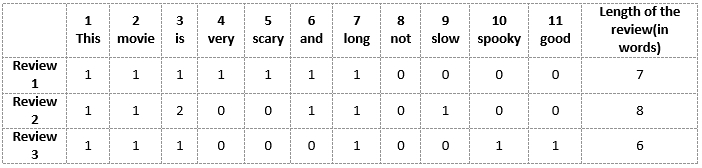
\includegraphics[height=2.4cm, width=12cm]{BOW_table}\\
Vector of Review 1: [1 1 1 1 1 1 1 0 0 0 0] \\
Vector of Review 2: [1 1 2 0 0 1 1 0 1 0 0] \\
Vector of Review 3: [1 1 1 0 0 0 1 0 0 1 1]
\end{flushleft}
\end{frame}

\begin{frame}{Contd ...}
\begin{flushleft}
In this approach, each word or token is called a "gram". Creating a vocabulary of two-word pairs is called a bigram model. \\
For example, the bigrams in the first document : "This movie is very scary and long" are as follows:\\
"This movie"\\
"movie is"\\
"is very"\\
"very scary"\\
"scary and"\\
"and long"\\
The process of converting NLP text into numbers is called vectorization in ML. Different ways to convert text into vectors are:
	\begin{itemize}
		\item Counting the number of times each word appears in a document.
		\item Calculating the frequency that each word appears in a document out of all the words in the document. 
	\end{itemize}
\end{flushleft}
\end{frame}

\begin{frame}{K-Nearest Neighbors}
\begin{flushleft}
		The k-NN algorithm is arguably the simplest machine learning algorithm. Building the model consists only of storing the training dataset. To make a prediction for a new data point, the algorithm finds the closest data points in the training dataset—its "nearest neighbors."
\myheading{k-Neighbors classification}
In its simplest version, the k-NN algorithm only considers exactly one nearest neigh‐
bor, which is the closest training data point to the point we want to make a prediction
for. The prediction is then simply the known output for this training point.
\end{flushleft}
\end{frame}

\begin{frame}{Contd...}
\begin{flushleft}
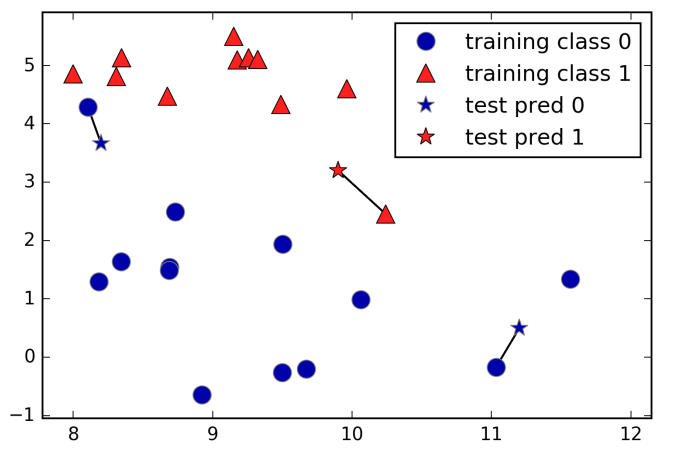
\includegraphics[height= 6.2cm, width=12cm]{KNN_example1}\\
		Here, we added three new data points, shown as stars. For each of them, we marked the closest point in the training set. The prediction of the one-nearest-neighbor algorithm is the label of that point.
\end{flushleft}
\end{frame}

\begin{frame}{Contd...}
\begin{flushleft}
\begin{itemize}
	\item Instead of considering only the closest neighbor, we can also consider an arbitrary number, k, of neighbors.
	\item This is where the name of the k-nearest neighbors algorithm comes from. When considering more than one neighbor, we use voting to assign a label.
	\item This means that for each test point, we count how many neighbors belong to class 0 and how many neighbors belong to class 1.
	\item We then assign the class that is more frequent: in other words, the majority class among the k-nearest neighbors.
\end{itemize}
	\end{flushleft}
\end{frame}

\begin{frame}{Contd...}
\begin{flushleft}
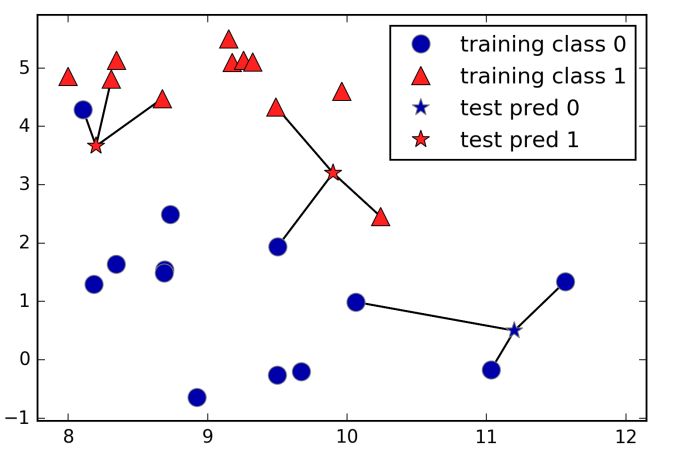
\includegraphics[height= 5.3cm, width=12cm]{KNN_example2}\\
	 We can see that the prediction for the new data point at the top left is not the same as the prediction when we used only one neighbor.
This illustration is for a binary classification problem, but it can be applied to datasets with any number of classes, for that we count how many neighbors belong to each class and again predict the most common class.
	\end{flushleft}
\end{frame}

\begin{frame}{Contd...}
\begin{flushleft}
\myheading{k-Neighbors regression}k=1
	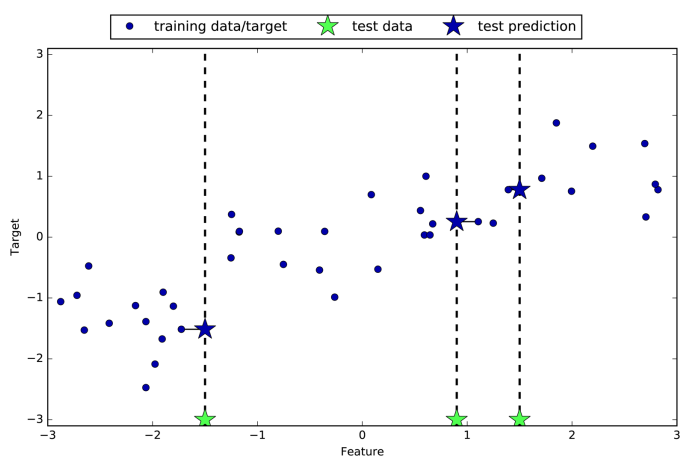
\includegraphics[height= 6.7cm, width=12cm]{KNN_example3}\\
	\end{flushleft}
\end{frame}

\begin{frame}{Contd...}
\begin{flushleft}
k=3
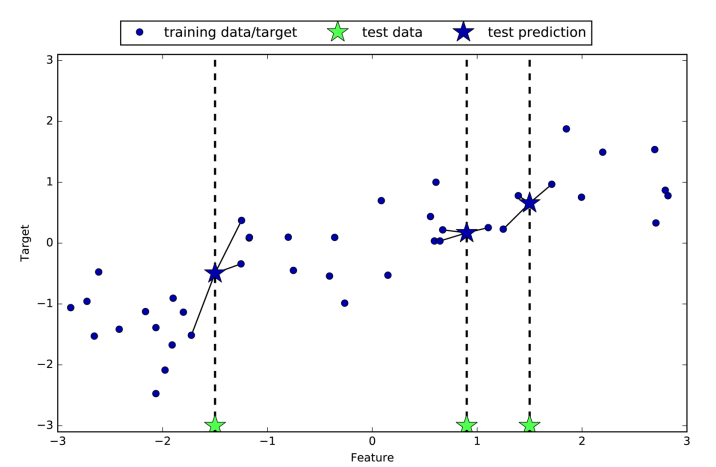
\includegraphics[height= 6.2cm, width=12cm]{KNN_example4}\\
When using
multiple nearest neighbors, the prediction is the average, or mean, of the relevant neighbors.
	\end{flushleft}
\end{frame}
\begin{frame}{Strengths, Weaknesses and Parameters of KNN}
\begin{flushleft}
\myheading{Strengths:}
	\begin{itemize}
		\item Model is very easy to understand, and often gives reasonable performance without a lot of adjustments.
		\item Versatile and Fast with smaller datasets and less number of features. 
	\end{itemize}
\myheading{Weaknesses:}
	\begin{itemize}
	\item When the training set is very large (either in number of features or in number of samples) prediction can be slow.
	\item Does not perform well on datasets with many features
	(hundreds or more), and it does particularly badly with datasets where most features are 0 most of the time (so called sparse datasets).
	\end{itemize}
\myheading{Parameters:}
	\begin{itemize}
		\item Number of neighbors (n\_neighbors)
		\item Distance metric (metric)
	\end{itemize}
\end{flushleft}
\end{frame}
\begin{frame}{Math behind KNN}
	\begin{flushleft}
		KNN falls in the supervised learning family of algorithms. More formally, our goal is to learn a function $h:X \rightarrow Y$ so that given an unseen observation $x$, $h(x)$ can confidently predict the corresponding output $y$.
		The KNN classifier is also a non parametric and instance-based learning algorithm.
\begin{itemize}
	\item \textbf{Non-parametric} means it makes no explicit assumptions about the functional form of h, avoiding the dangers of mismodeling the underlying distribution of the data.
	\item \textbf{Instance-based} learning means that our algorithm doesn’t explicitly learn a model. Instead, it chooses to memorize the training instances which are subsequently used as “knowledge” for the prediction phase. Concretely, this means that only when a query to our database is made (i.e. when we ask it to predict a label given an input), will the algorithm use the training instances to spit out an answer.
\end{itemize}
	\end{flushleft}
\end{frame}
\begin{frame}{Similarity measures in KNN}
	\begin{flushleft}
	Similarity is defined according to a distance metric between two data points. Distance metrics used in KNN includes:
		\begin{itemize}
			\item \textbf{Euclidean Distance: } $ d(x, x') = \sqrt{\sum\limits_{i=1}^n{\left(x_i - x'_i \right)^2}}$
			\item \textbf{Manhattan Distance: } $ d(x, x') = \sum\limits_{i=1}^n{|x_i - x'_i|}$
			\item \textbf{Minkowski Distance: } $ (\sum\limits_{i=1}^n{|x_i - y_i|^p})^{1/p}$
			\item \textbf{Cosine Distance: } $ \cos(\theta )={\vec{a} \cdot \vec{b}  \over \|\vec{a} \|\|\vec{b} \|}$
			\item \textbf{Hamming Distance}
			\item \textbf{Chebyshev Distance}
			\item \textbf{Mahalanobis Distance}
		\end{itemize}
	\end{flushleft}
\end{frame}

\begin{frame}{KNN Working}
	\begin{flushleft}
		Given a positive integer $K$, an unseen observation $x$ and a similarity metric $d$, KNN classifier performs the following two steps:
\begin{itemize}
	\item It runs through the whole dataset computing d between $x$ and each training observation. We’ll call the $K$ points in the training data that are closest to $x$ the set $A$. Note that $K$ is usually odd to prevent tie situations.
	\item It then estimates the conditional probability for each class, that is, the fraction of points in $A$ with that given class label. (Note $I(x)$ is the indicator function which evaluates to $1$ when the argument $x$ is true and $0$ otherwise)
\end{itemize}
	\begin{equation*}
	P(y = j | X = x) = \frac{1}{K} \sum\limits_{i \in \mathcal{A}} I(y^{(i)} = j)
	\end{equation*}
	Finally, our input $x$ gets assigned to the class with the largest probability.\\
	An alternate way of understanding KNN is by thinking about it as calculating a decision boundary (i.e. boundaries for more than 2 classes) which is then used to classify new points.
\end{flushleft}
\end{frame}
\begin{frame}
\huge{\centerline{The End}}
\end{frame}
\end{document}